%% Be sure to check spelling!

%% Put your name and the proper due date in place

%% Note that the \includegraphics and \lstinputlisting commands
%% are currently commented out with %%% - until the
%% files exist, processing this code without them will result in an error
%% so leave the comments until you have created the files!

\documentclass{article}
\usepackage{amsmath}    % loads AMS-Math package
\usepackage{graphicx}   % bring in graphics
\usepackage{listings}   % allows lstlisting environment
\usepackage{moreverb}   % allows listinginput environment
\usepackage[letterpaper, margin=0.5in]{geometry}  % set paper size/margins
\usepackage{EGR103style}  % colorful file imports

\begin{document}
\begin{center}
\rule{6.5in}{0.5mm}\\~\\
\textbf{\large EGR 103L -- Fall 2021}\\~\\
\textbf{\huge Laboratory 12 - Interpolations}\\~\\
**NAME (NET ID)**\\
Lab Section **Section**, **DAY AND TIMES**\\
**DATEDUE**, **YEAR**\\~\\
{\small I have adhered to the Duke Community Standard in completing this assignment.  I understand that a violation of the Standard can result in failure of this assignment, failure of this course, and/or suspension from Duke University.} 
\rule{6.5in}{0.5mm}\\
\end{center}
\tableofcontents
\listoffigures
\clearpage

\appendix
\section{Codes}
% Put the name of your file in the subsection name 
% and the listinginput input
% Be sure to include the community standard in codes!
% Add \pagebreaks if they make sense
% Make as many copies as you need
\lstset{style=python103, language=python} 

\subsection{Chapra 18.9}
%%%\lstinputlisting{chapra_18_009.py}
\clearpage 

\subsection{Chapra 18.10}
%%%\lstinputlisting{chapra_18_010.py}
\clearpage

\subsection{Chapra 18.14}
%%%\lstinputlisting{chapra_18_014.py}
\clearpage

\section{Figures}
% Make as many as needed; change sizes if it makes sense to do so
\begin{figure}[h!]
\begin{center}
%%%\includegraphics{chapra_18_009_plot.png}
\caption{Chapra 18.9}
\end{center}
\end{figure}

\begin{figure}[h!]
\begin{center}
%%%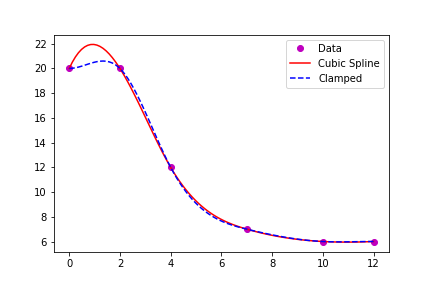
\includegraphics{chapra_18_010_plot.png}
\caption{Chapra 18.10}
\end{center}
\end{figure}

\end{document}